\section{8.8. Dealing with Scale}

\begin{frame}{Nội dung trình bày}
	\tableofcontents[currentsection]
\end{frame}

% SLIDE: 8.8.1 Scaling Laws
\begin{frame}{8.8.1. Scaling Laws}
	\textbf{Hiệu năng (Loss)} của các LLM phụ thuộc vào 3 yếu tố chính:
			\begin{itemize}
				\item \textbf{Model size (N):} số lượng tham số của mô hình.
				\item \textbf{Dataset size (D):} kích thước tập dữ liệu huấn luyện.
				\item \textbf{Compute (C):} tổng tài nguyên tính toán.
			\end{itemize}
	\vspace{0.4cm}
	Mối quan hệ giữa hiệu năng và 3 yếu tố này còn được gọi là \textbf{scaling laws}.

\end{frame}

\begin{frame}{8.8.1 Scaling Laws}
	\textbf{Kaplan et al. (2020)} đưa ra công thức về mối quan hệ giữa Loss $L$ với số lượng tham số non-embedding $N$, kích thước tập dữ liệu huấn luyện $D$ và tài nguyên tính toán $C$:
	\begin{align*}
		L(N) &= \left( \frac{N_c}{N} \right)^{\alpha_N} \tag{8.49} \\[10pt]
		L(D) &= \left( \frac{D_c}{D} \right)^{\alpha_D} \tag{8.50} \\[10pt]
		L(C) &= \left( \frac{C_c}{C} \right)^{\alpha_C} \tag{8.51}
	\end{align*}
\end{frame}

\begin{frame}{8.8.1 Scaling Laws}
Đối với thí nghiệm của \textbf{Kaplan et al. (2020)}, các giá trị cụ thể được xác định là:

\begin{itemize}
	\item $\alpha_N = 0.076,\quad N_c = 8.8 \times 10^{13}$ parameters
	\item $\alpha_D = 0.095,\quad D_c = 5.4 \times 10^{13}$ tokens
	\item $\alpha_C = 0.050,\quad C_c = 3.1 \times 10^{8}$ petaflop-days
\end{itemize}

\vspace{0.3cm}



\end{frame}

\begin{frame}{8.8.1 Scaling Laws}
	
	Hoffmann et al (2022):
	
	\vspace{0.2cm}
	
	\renewcommand{\arraystretch}{1.2}
	\resizebox{\textwidth}{!}{
		\begin{tabular}{lcc}
			\hline
			\textbf{Approach} & \textbf{Coeff. $a$ where $N_{\text{opt}} \propto C^a$} & \textbf{Coeff. $b$ where $D_{\text{opt}} \propto C^b$} \\
			\hline
			1. Minimum over training curves & 0.50 (0.488, 0.502) & 0.50 (0.501, 0.512) \\
			2. IsoFLOP profiles & 0.49 (0.462, 0.534) & 0.51 (0.483, 0.529) \\
			3. Parametric modelling of the loss & 0.46 (0.454, 0.455) & 0.54 (0.542, 0.543) \\
			\hline
			Kaplan et al. (2020) & 0.73 & 0.27 \\
			\hline
		\end{tabular}
	}
\end{frame}

\begin{frame}{8.8.1 Scaling Laws}
	\textbf{Số lượng tham số $N$} có thể được ước lượng gần đúng từ các thành phần kiến trúc của Transformer:

	\begin{align*}
		N &\approx 2\ d\ n_{\text{layer}}(2 d_{\text{attn}} + d_{\text{ff}}) \\
		&\approx 12\ n_{\text{layer}} d^2 \tag{8.52} \\
		&\text{(giả sử } d_{\text{attn}} = d_{\text{ff}}/4 = d\text{)}
	\end{align*}

	
	\vspace{1em}
	\textbf{Trong đó:} 
	\begin{itemize}
		\item $d$: chiều input-output, $d_{\text{attn}}$: chiều self-attention, $d_{\text{ff}}$: chiều feedforward.
		\item Số tham số tăng rất nhanh khi tăng chiều rộng ($d^2$) và số lớp ($n_{\text{layer}}$).
	\end{itemize}
\end{frame}

\begin{frame}{8.8.1 Scaling Laws}

	Scaling laws hữu dụng trong các trường hợp sau:
	\begin{itemize}
		\item \textbf{Tối ưu hóa huấn luyện:} Xác định cách cấu hình mô hình để đạt mức performance mong muốn.
		\item \textbf{Dự báo hiệu năng:} Dự đoán sự thay đổi của Loss khi tăng quy mô dữ liệu hoặc tham số.
		\item \textbf{Cân bằng Data \& Model:} Ước lượng lượng dữ liệu cần thiết khi scale-up, tránh việc tăng tham số một cách "mù quáng".
		\item \textbf{Tiết kiệm chi phí:} Sử dụng các thí nghiệm nhỏ để dự đoán hành vi của mô hình lớn, giảm thiểu rủi ro tài chính.
	\end{itemize}
\end{frame}


\begin{frame}{8.8.2 KV Cache}
	Khi huấn luyện, Attention được tính toán song song rất hiệu quả qua phép nhân ma trận:
	\begin{equation*}
		\mathbf{A} = \text{softmax}\left(\frac{\mathbf{QK}^\top}{\sqrt{d_k}}\right)\mathbf{V} \tag{8.53}
	\end{equation*}
	
	Việc tính toán Attention trong inference (suy luận) xảy ra vấn đề gì?
 
	\pause
	
	\begin{itemize}
		\item Các token được tạo ra \textbf{tuần tự} từng cái một.
		\item Với mỗi token mới $\mathbf{x}_i$, ta cần tính các vector $Q, K, V$.
		\item Việc tính toán lại $K$ và $V$ cho tất cả các token trước đó ($\mathbf{x}_{<i}$) là cực kỳ lãng phí tài nguyên và thời gian.
	\end{itemize}

\end{frame}

\begin{frame}{8.8.2 KV Cache}
KV Cache giúp tối ưu hóa quá trình suy luận (inference) bằng cách tránh các tính toán dư thừa:
	\vspace{1em}
\begin{itemize}
	\item Thay vì tính toán lại từ đầu, ta sẽ \textbf{lưu trữ lại} các giá trị \textbf{Key và Value} của các token trước đó vào cache.
	\vspace{0.5em}
	\item Khi một token mới được sinh ra, mô hình chỉ cần thực hiện tính toán bộ ba $QKV$ cho \textbf{duy nhất token đó}. 
	\vspace{0.5em}
	\item Sau đó, nó sẽ kết hợp với các \textbf{Key và Value} đã được \textbf{lưu trong cache} để hoàn tất phép toán Attention.

\end{itemize}
\end{frame}

\begin{frame}{8.8.2 KV Cache}
\begin{figure}
	\centering
	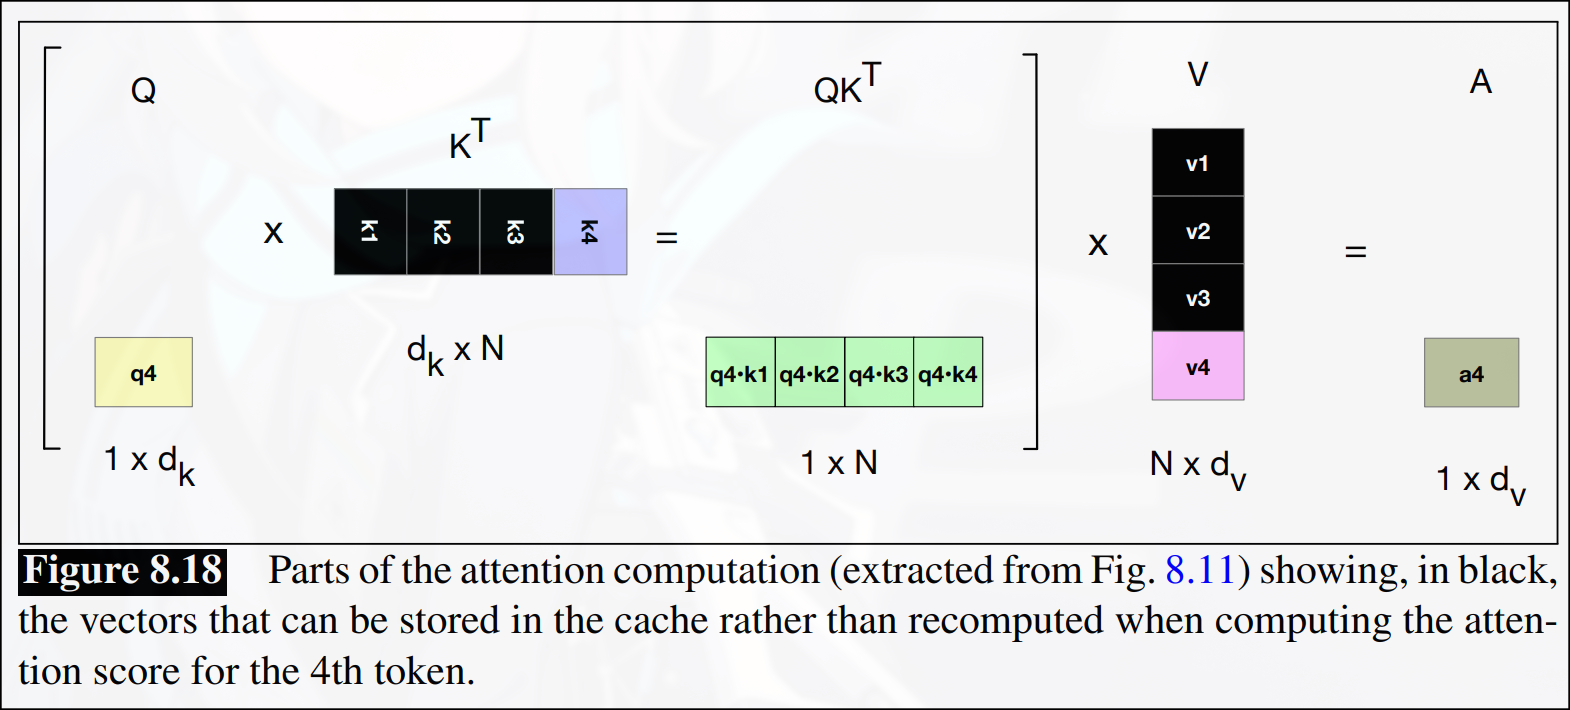
\includegraphics[width=1.0\linewidth]{img/figure8_18}
\end{figure}

\end{frame}


\begin{frame}{8.8.3 Parameter Efficient Fine Tuning (PEFT)}

	Mô hình pretrained thường được finetune trên dữ liệu domain mới để học thêm kiến thức chuyên biệt.
	
	\vspace{0.5em}
	Tuy nhiên, full finetuning trên LLM rất tốn bộ nhớ, compute và thời gian vì \textbf{số tham số quá lớn}.
	
	\vspace{0.8em}

	$\Rightarrow$ Từ đó xuất hiện các phương pháp chỉ finetune \textbf{một phần nhỏ tham số} thay vì thay đổi toàn bộ, và nhóm phương pháp này được gọi là \textbf{parameter-efficient fine tuning (PERT)}.
\end{frame}

\begin{frame}{8.8.3 Parameter Efficient Fine Tuning (PEFT)}
	\textbf{LoRA (Low-Rank Adaptation)} là một phương pháp thuộc nhóm PEFT.

\vspace{0.5em}
Ý tưởng chính của LoRA là, thay vì cập nhật trực tiếp các ma trận lớn trong Transformer, LoRA giữ nguyên chúng và chỉ học thêm \textbf{một phần hiệu chỉnh nhỏ}.

\vspace{0.5em}
Nhờ vậy, số tham số cần huấn luyện giảm mạnh, giúp tiết kiệm bộ nhớ, compute và thời gian so với full finetuning.
\end{frame}

\begin{frame}{8.8.3 Parameter Efficient Fine Tuning (PEFT)}
	\setlength{\columnsep}{0.3cm}
	
	\begin{columns}[T,onlytextwidth]
		
		\column{0.4\textwidth}
		\textbf{Cập nhật thông thường}
		
		Giả sử ma trận cần finetune là
		\[
		W \in \mathbb{R}^{k \times d}
		\]
		
		Ta cập nhật trực tiếp:
		\[
		\Delta W \in \mathbb{R}^{k \times d}
		\]
		
		Ma trận sau khi cập nhật:
		\[
		W + \Delta W
		\]
		
		Phép biến đổi đầu ra:
		\[
		h = xW
		\]
		
		\column{0.02\textwidth}
		\centering
		\vspace{0.3cm}
		\rule{0.4pt}{0.65\textheight}
		
		\column{0.47\textwidth}
		\textbf{Cập nhật bằng LoRA}
		
		Đóng băng $W$ và học hai ma trận hạng thấp:
		\[
		A \in \mathbb{R}^{k \times r}, \quad
		B \in \mathbb{R}^{r \times d}
		\]
		\[
		r \ll \min(k,d)
		\]
		
		\vspace{0.5cm}
		Thay vì học $\Delta W$, LoRA dùng:
		\[
		W + \Delta W \approx W + AB
		\]
		
		Phép biến đổi đầu ra trở thành:
		\begin{equation}
			h = xW + xAB
			\tag{8.54}
		\end{equation}
		
	\end{columns}
\end{frame}
\begin{frame}{8.8.3 Parameter Efficient Fine Tuning (PEFT)}
\begin{figure}
	\centering
	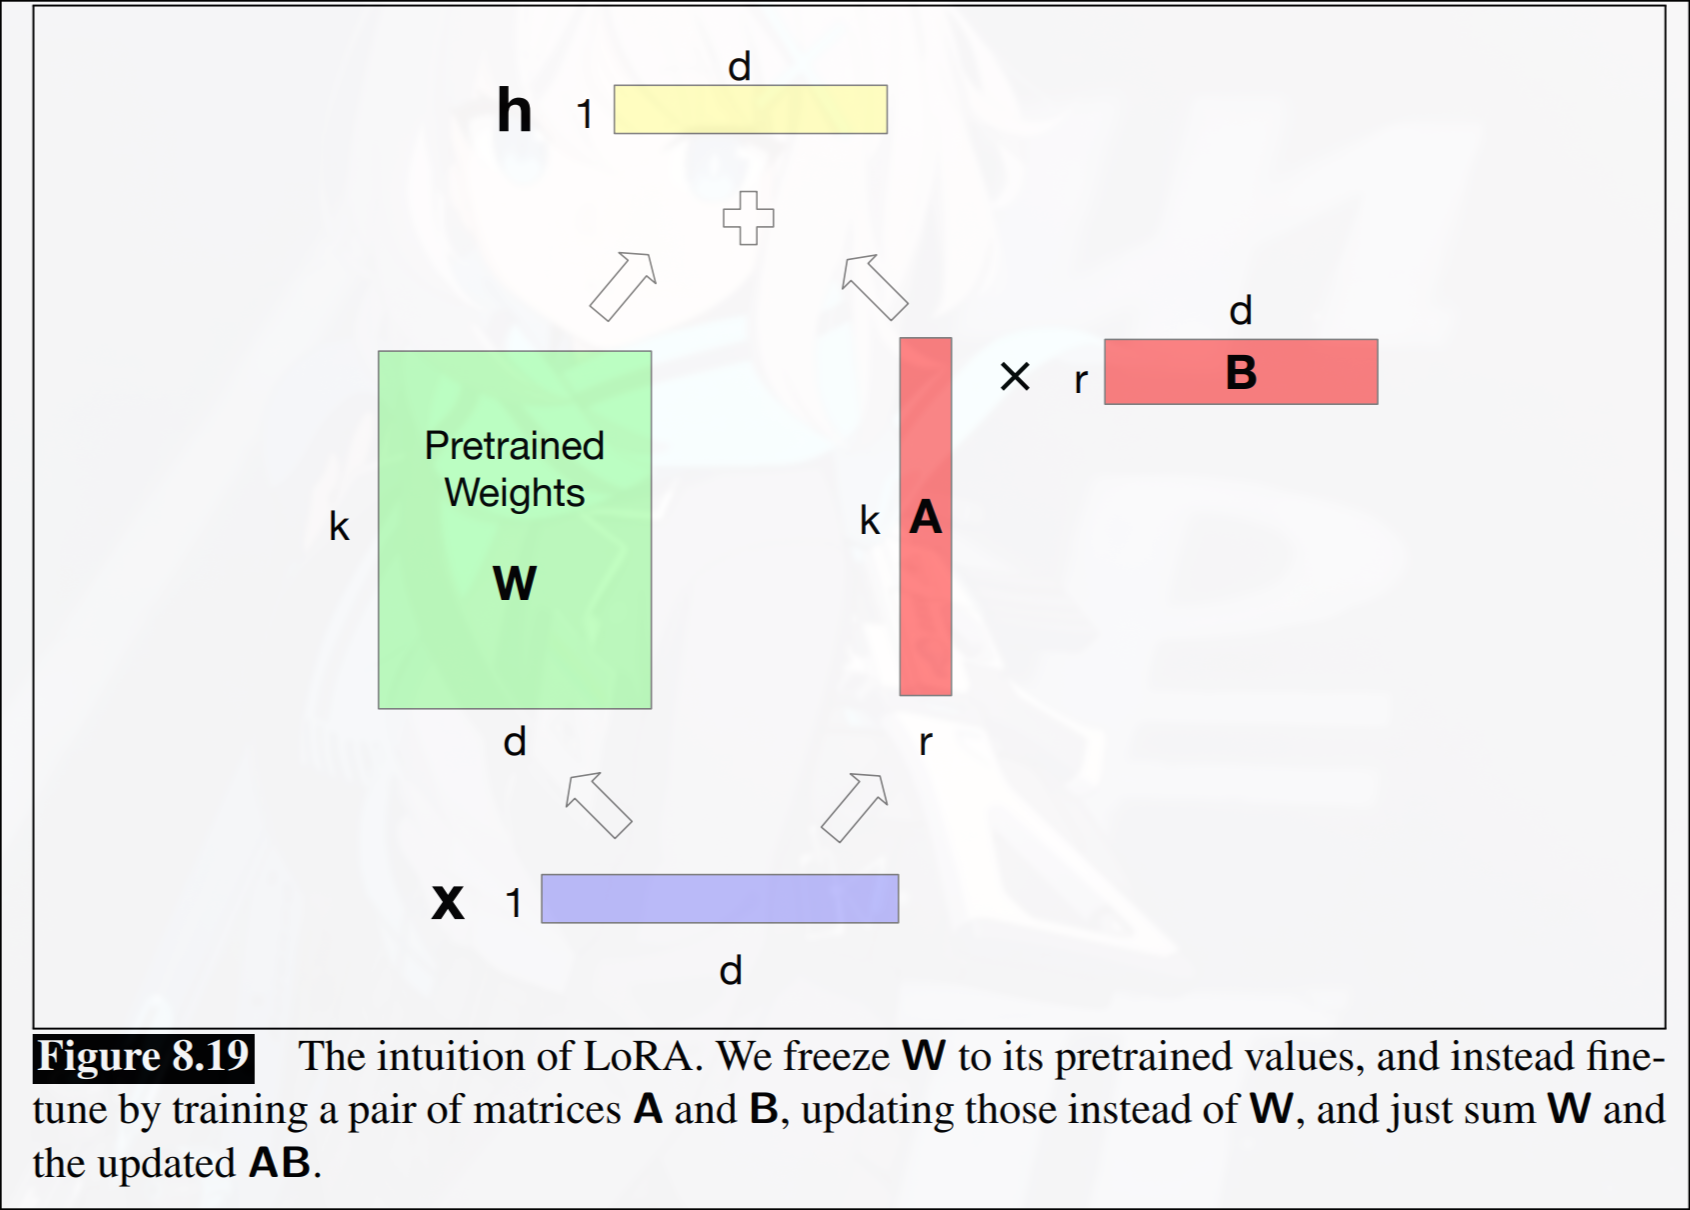
\includegraphics[width=0.9\linewidth]{img/figure8_19}

\end{figure}
\end{frame}


\begin{frame}{8.8.3 Parameter Efficient Fine Tuning (PEFT)}
\scriptsize
\renewcommand{\arraystretch}{1.2}

\begin{table}[h]
	\centering
	\resizebox{\textwidth}{!}{
		\begin{tabular}{|p{1.8cm}|p{3.9cm}|p{3.3cm}|p{3.3cm}|}
			\hline
			\textbf{Phương pháp} & \textbf{Cách làm} & \textbf{Ưu điểm} & \textbf{Nhược điểm} \\
			\hline
			LoRA & Đóng băng trọng số gốc, chỉ học hai ma trận hạng thấp để biểu diễn phần cập nhật của trọng số & Hiệu quả tốt, ít tham số cần học, phổ biến, suy luận gần như không bị tăng độ trễ nhiều & Vẫn cần backbone ở precision tương đối cao nếu không kết hợp lượng tử hóa \\
			\hline
			QLoRA & Lượng tử hóa backbone xuống 4-bit rồi gắn LoRA để fine-tune & Tiết kiệm VRAM rất mạnh, phù hợp khi tài nguyên phần cứng hạn chế, vẫn giữ hiệu năng tốt & Pipeline phức tạp hơn, phụ thuộc vào quantization và thư viện hỗ trợ \\
			\hline
			Prompt Tuning & Giữ nguyên mô hình, chỉ học một số soft prompt gắn vào đầu vào để dẫn hướng mô hình & Rất ít tham số cần học, đơn giản, phù hợp với mô hình rất lớn & Thường kém ổn định hơn LoRA, hiệu quả phụ thuộc mạnh vào task và thiết kế prompt \\
			\hline
			IA3 & Học các vector scale nhỏ để điều chỉnh activation trong attention và feed-forward & Rất ít tham số, hiệu quả khá tốt, gọn hơn nhiều so với fine-tune toàn bộ & Ít trực quan hơn Adapter, mức linh hoạt và phổ biến thực tế thường không bằng LoRA \\
			\hline
		\end{tabular}
	}
\end{table}
\end{frame}